\chapter{Qubit calibration}

In this chapter I will describe the process of calibration for superconducting flux-tunable transmon on the hardware located in the QRC (Quantum Research Center) Laboratory of the TII (Technology \& Innovation Institute) in Abu Dhabi.

\section{Experimental setup}
All the results presented in this work were obtained using the Contralto-D chip \cite{qw11q}, which offers up to 21 fully connected qubits and 4 isolated qubits, for a total of 25 physical qubits.
The distinction between fully connected and isolated qubits is important as only the fully connected subset supports direct two-qubit gate operations, which are essential for implementing entangling gates and complex quantum circuits. 
Isolated qubits, while still operational for single-qubit tasks, do not participate in multi-qubit interactions and thus are not functionally equivalent in terms of computational capabilities.
The topology of the qubit is shown in figure \ref{fig:qw11q_topology}.

\begin{figure}[ht!]
    \centering
    \begin{subfigure}{0.40\textwidth}
        \centering
        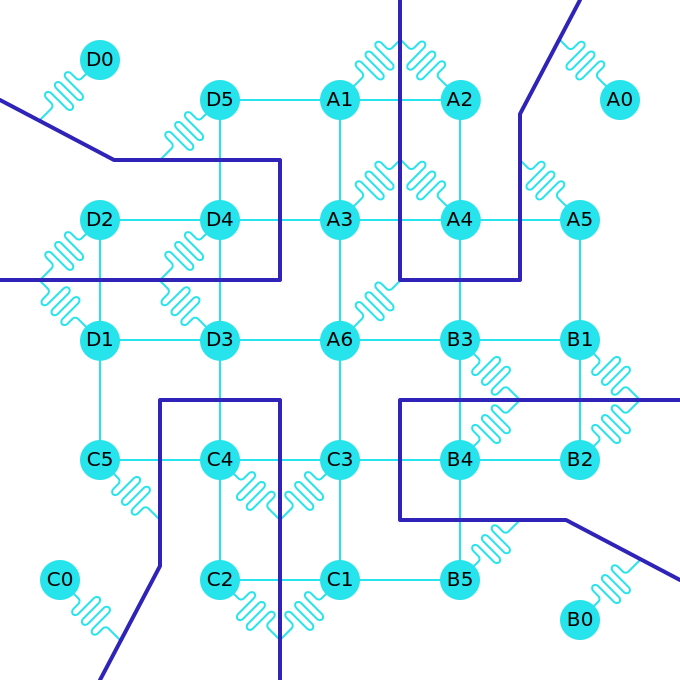
\includegraphics[width=0.80\textwidth]{figures/png/qw11q.jpeg}
        \subcaption{}
        \label{fig:qw11q_picture}
    \end{subfigure}
    \hfill
    \begin{subfigure}{0.50\textwidth}
        \centering
        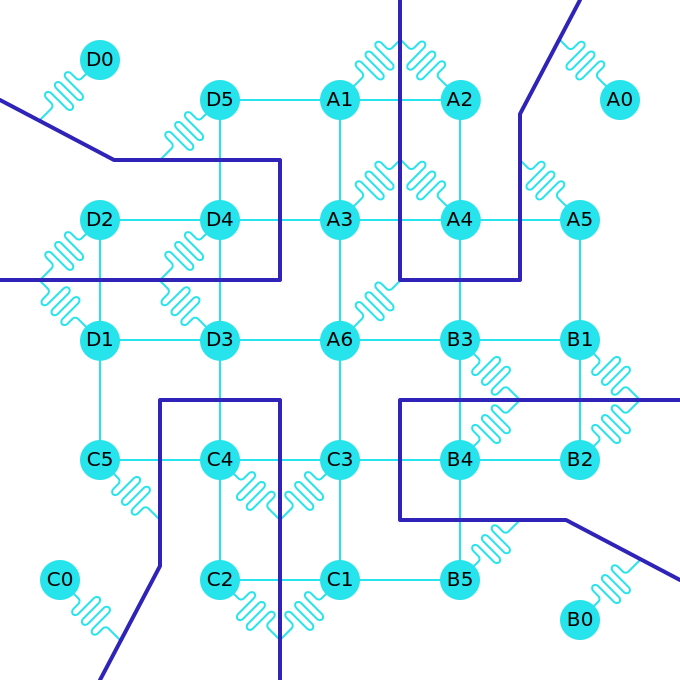
\includegraphics[width=\textwidth]{figures/png/qw11q.png}
        \subcaption{}
        \label{fig:qw11q_topology}
    \end{subfigure}
    \caption{Figure \ref{fig:qw11q_picture}: Picture of the Contralto-D chip from QuantWare. Figure \ref{fig:qw11q_topology}: Topology of the Contralto-D chip from QuantWare.}
    \label{fig:qw11q}
\end{figure}

As discussed in the previous chapter, the behavior of Josephson junctions and SQUIDs relies critically on the superconducting state of the materials involved. 
To achieve and maintain this regime, it is essential that the superconducting elements operate well below their critical temperature. 
For this reason, the Contralto-D chip is installed at the lowest temperature stage of the cryostat, where the required thermal conditions for superconductivity are met. 
This ensures the proper functioning of the quantum hardware and enables the realization of coherent quantum operations.

These systems achieve ultra-low temperatures by exploiting the unique quantum properties of helium-3 (\ce{^{3}He}) and helium-4 (\ce{^{4}He}) isotopes in a dilution process.
At the core of a dilution refrigerator is a mixing chamber, where the cooling mechanism takes place. 
When a mixture of \ce{^{3}He} and \ce{^{4}He} is cooled below approximately 870 millikelvin, the two isotopes phase-separate into a \ce{^{3}He}-rich phase and a \ce{^{3}He}-dilute phase. 
The key principle is that when \ce{^{3}He} atoms cross the phase boundary—from the concentrated phase into the dilute phase—they absorb energy from their surroundings. 
This process is endothermic and is the fundamental source of cooling in the dilution refrigerator.\\
The system operates as a closed loop: \ce{^{3}He} gas is circulated using a combination of sorption pumps and still pumps, which remove \ce{^{3}He} vapor from the still (typically at $600–800$ mK), recondense it at a higher stage, and reintroduce it into the mixing chamber. 
The refrigerator includes several thermalization stages—typically at $50$ K, $4$ K, $800$ mK, $100$ mK, and finally below $20$ mK—each connected to a corresponding cooling stage and separated by radiation shields and thermal filters to minimize heat load and noise from higher-temperature stages.
Dilution refrigerators are highly stable and capable of reaching base temperatures below $10$ mK, with hold times on the order of days or even weeks. 
These temperatures are crucial for achieving the low thermal noise and long coherence times necessary for high-fidelity quantum operations in superconducting circuits.
Specifically the cryostat employed in the lab is the XLDsl from Bluefors \cite{XLD1000}, an image of the cryostat is shown in figure \ref{fig:XLDsl}.

\begin{figure}[h!]
    \centering
    \includegraphics[width=0.35\textwidth]{figures/png/XLD1000.png}
    \caption{Picture of the XLDsl dilution refrigerator at the QRC Lab}
    \label{fig:XLDsl}
\end{figure}

Outside the cryostat, the control and readout of superconducting qubits are managed by dedicated room-temperature electronics.
These systems are responsible for generating the microwave pulses used to drive single- and two-qubit gates, as well as for acquiring and processing the output signals that encode the qubit states 
Typically they include arbitrary waveform generators (AWGs), microwave sources, mixers, digitizers, and field-programmable gate arrays (FPGAs).
The generated microwave pulses are shaped and modulated at room temperature before being attenuated and routed to the cryogenic environment. 
Similarly, signals returning from the qubits are amplified and digitized for state discrimination and further processing. 
The electronics employed in the lab for the control of the \tt{qw11q} is the OPX1000 platform by Quantum Machines \cite{opx1000}.

The software I used for the calibration of the qubits and the subsequent experiments is \Qibocal (\cite{pasquale_qibocal_2024}, \cite{qibocalscience}, \cite{qibocalgit}), while the backend for communication with the laboratory instruments is \Qibolab (\cite{efthymiou_qibolab_2024}, \cite{qibolabscience}, \cite{qibolabgit}).
\Qibolab is the control layer responsible for managing and executing low-level instructions on the hardware, bridging high-level quantum models and physical quantum platforms.
It is designed to support diverse experimental setups and allows the researcher to define custom hardware configurations through a platform abstraction and to execute custom pulse sequences using both commercial and open-source firmware.
The communication between \Qibolab and the quantum hardware is structured and modular, relying on a stack that includes instrument drivers, pulse control logic, and a compiler that translates abstract quantum gates into hardware-specific instructions.
This structure enables compatibility with heterogeneous platforms and facilitates the development of experimental drivers tailored to different laboratory environments.
\Qibocal interfaces directly with \Qibolab to apply calibration protocols on the physical device. The routines deployment takes place through the interpretation of declarative runcards written in YAML.
\Qibocal allows an easy execution of pulse sequences, collection of measurement data, and interpretation of the results through the reports that are automatically generated upon completion of the routine.

\section{Single qubit calibration experiments}

The first task that I needed to complete at the beginning of my thesis work was the calibration of at least a line of the superconducting quibts of the Contralto-D chip using the \Qibocal library.
From this point onward, for the sake of brevity, I will refer to the chip interchangeably as Contralto-D or \tt{qw11q}, which is the name of the node under which it is registered on the QRC computing cluster.
In the following I will describe the experiments that I performed and commenting on the results.

\subsection{Resonator characterization}

\subsubsection{Resonator spectroscopy}
The first step to calibrate the readout pulse is to charachterize the resonator is to find the resoinator frequency, that is the tranisition frequency for the resonator. 
At this frequency, a distinct difference in the transmitted signal can be observed depending on the type of resonator used. 
In the case of a 3D cavity resonator, the signal appears amplified, whereas for a 2D planar resonator, the signal tends to be more strongly absorbed. Regardless of the resonator type, the response typically exhibits a Lorentzian-shaped peak: this peak is positive for 3D cavities due to the amplification effect, and negative for 2D resonators due to their greater absorption.

The outcome of this experiment is strongly influenced by the amplitude of the excitation pulse. 
To reliably determine the resonator frequency, the pulse duration can be fixed on the order of microseconds, which is sufficient to observe the relevant signal response.
However, selecting an appropriate amplitude requires more careful consideration. When the amplitude is high, the signal becomes more prominent, improving the signal-to-noise ratio and making it easier to identify the resonator's response.
If the amplitude is increased too much, however, it can drive the system out of the superconducting regime.  In this case, the resonator becomes effectively decoupled from the qubit, and the frequency observed corresponds to the so-called bare resonator frequency.
An example of measurement of the bare resonator frequency is shown in Figure \ref{fig:res_high}.
 
\begin{figure}[h!]
    \centering
    \includegraphics[width=\textwidth]{figures/png/res_spectroscopy_high.png}
    \caption{Output of resonator spectroscopy with high power on qubit B2.}
    \label{fig:res_high}
\end{figure}

Una misura della frequenza di risonanza del resonator low power è invece riportato in Figure \ref{fig:res_low}

\begin{figure}[h!]
    \centering
    \includegraphics[width=\textwidth]{figures/png/res_low.png}
    \caption{Output of resonator spectroscopy with low power on qubit B2.}
    \label{fig:res_low}
\end{figure}

Uno studio più preciso della risposta del risonatore può essere realizzato eseguendo la routine di resonator spectroscopy cambiando la funzione di fit,  questa variazione dell'esperimento è descritta nell'appendice \hyperref[app:AppendixA]{Appendix A}

\subsubsection{Resonator punchout}
To identify the resonator frequency under qubit coupling, it is necessary to first determine the appropriate readout pulse amplitude. 
This can initially be explored using a vector network analyzer to verify system functionality and obtain a rough estimate of the relevant parameters. 
Then it is possible to repeat the spectroscopy, this time over a narrower frequency range and for varying pulse amplitudes. 
The resonator frequency is expected to depend strongly on amplitude: it remains constant in the high-power regime, shifts during an intermediate transition phase, and stabilizes again at a different value once the qubit-resonator interaction becomes significant.

%The expected result from a resonator punchout experiment is shown in Figure \ref{fig:res_punchout}
%\begin{figure}[h!]
%    \centering
%    \includegraphics[width=\textwidth]{figures/png/}
%    \caption{Output of resonator punchout on qubit B2.}
%    \label{fig:res_punchout}
%\end{figure}

\subsubsection{Resonator flux dependence}


\subsubsection{Resonator crosstalk}

\subsection{Qubit characterization}
Dopo aver calibrato e ricavato i parametri del risonatore accopiato al qubit è possibile procedere con la calibrazione dei parametri relativi al qubit stesso.

\subsubsection{Qubit spectroscopy}
To determine the resonance frequency of a qubit, a qubit spectroscopy experiment is performed, which, unlike resonator spectroscopy, requires a two-tone approach. 
While resonator spectroscopy is typically a single-tone measurement used to identify the resonator's response, qubit spectroscopy involves applying a drive tone to the qubit followed by a readout tone to detect the qubit state. 
This method becomes essential after an initial estimate of the readout frequency and amplitude has been obtained from a resonator punchout experiment. 
In this protocol, a drive pulse of variable frequency $\omega$ is sent through the qubit drive line. 
If the drive frequency is far detuned from the qubit transition frequency $\omega_{q}$, it will have no appreciable effect on the qubit state, and the measured signal will remain unchanged. 
However, as $\omega$ approaches $\omega_{01}$ the drive pulse can induce transitions between the qubit states. 
This excitation modifies the qubit population and, consequently, the resonator response, which is sensitive to the qubit state due to their dispersive coupling. 
When the drive frequency is near resonance and the pulse is sufficiently long, the qubit may reach a maximally mixed state leading to a detectable change in the readout signal amplitude. 
By sweeping the drive frequency and recording the corresponding readout amplitudes, one can plot a spectroscopy curve that reveals a Lorentzian dip or peak centered at the qubit transition frequency—opposite in direction to the Lorentzian feature observed in the resonator spectroscopy, due to the nature of the state-dependent dispersive shift.

An example of the output of qubit spectroscopy experiment is shown in figure \ref{fig:qubit_spectroscopy}
\begin{figure}[h!]
    \centering
    \includegraphics[width=\textwidth]{figures/png/qubit_spectroscopy.png}
    \caption{Output of qubit spectroscopy on qubit B2.}
    \label{fig:qubit_spectroscopy}
\end{figure}

\subsubsection{Qubit EF spectroscopy}
Qubit spectroscopy can also be extended to probe transitions to higher excited states beyond the first excited state. 
Directly observing these higher-level transitions typically requires significantly increased drive power, which may exceed the safe operational limits of the experimental setup. 
An alternative and more controlled approach involves first preparing the qubit in state $\ket{1}$, followed by a standard spectroscopy sequence to induce the $\ket{1} \leftrightarrow \bra{2}$ transition. 

%\begin{figure}[h!]
%    \centering
%    \includegraphics[width=\textwidth]{figures/png/ef.png}
%    \caption{Output of qubit spectroscopy to identify the transition frequency between state $\ket{1}$ ($\ket{e}$) and state $\ket{f}$ (first scited state) on qubit B2.}
%    \label{fig:ef}
%\end{figure}

Si noti che la descrizione di questa routine di calibrazione è stata inserita qui per una questione di chiarezza e continuità espositiva, tuttavia dato che richiede che il qubit all'inizio della spettroscopia si trovi nello stato $\ket{1}$ può essere eseguita solo dopo l'esecuzione di una single-shot classification\ref{subsec:single_shot}.

\subsubsection{Qubit flux dependence}

\begin{figure}[h!]
    \centering
    \includegraphics[width=\textwidth]{figures/png/qubit_flux.png}
    \caption{Output of the qubit flux dependence on qubit B2.}
    \label{fig:qubit_flux}
\end{figure}

\subsubsection{Qubit crosstalk}

\subsection{T1 \& T2 measurement}

\begin{figure}[h!]
    \centering
    \includegraphics[width=\textwidth]{figures/png/t1.png}
    \caption{Output of the $T1$ measurement on qubit B2.}
    \label{fig:t1}
\end{figure}

\begin{figure}[h!]
    \centering
    \includegraphics[width=\textwidth]{figures/png/t2_strange.png}
    \caption{Output of the $T2$ measurement on qubit B2.}
    \label{fig:t1}
\end{figure}

\subsection{Single shot classification}\label{subsec:single_shot}

\begin{figure}[h!]
    \centering
    \includegraphics[width=0.4\textwidth]{figures/png/classification.png}
    \caption{Output of the single shot classification on qubit B2.}
    \label{fig:t1}
\end{figure}

%eventualmente in appendice riportare il fatto che è possibile eseguirli anche direttamente sul segnale, senza aver bisogno della classificazione dello stato.
%semplicemente al posto della probabilità di trovarsi in un determinato stato verrà riportato direttamente il segnale di acquisizione dello strumento. 

\subsection{Gate calibration}
\subsubsection{Rabi amplitude}
\subsubsection{Rabi length}
\subsubsection{Rabi amplitude-length}

\subsection{Fine calibration}
\subsubsection{Ramsey experiment}
\subsubsection{Flipping experiment}
\subsubsection{Dispersive shift}
\subsubsection{Readout charachterization}

\subsection{Standard Randomized Benchmarking}
L'esperimento di standard randomized benchmarking verrà descritto più nel dettaglio nel capitolo successivo (see Section \ref{sec:RBsection}), per il momento basti sapere che 

\subsection{DRAG experiment}\label{sec:DRAG}
\cite{Motzoi_2009}\cite{Gambetta_2011}
%write a subsection for each experiment

